\chapter{Applications and experimental results}
\label{c:results}

\section{Examples}

Here we show several proof of concept examples for using the \emph{spexs2} tool.

\subsection{Genomic sequences}

The original SPEXS algorithm worked on genomic sequences, so it is appropriate to show that \emph{spexs2} also works on such datasets. Here is a problem that was presented in "Pattern Discovery in From Biosequences"\cite{spexs}. The search problem was to find overrepresented sequences from a cluster of co-expressed genes by comparing them to a set of random samples from upstream sequences in yeast genome.

\begin{file}
Pattern       Cluster    Background   Ratio      Binomial Prob.
GATGAG.T      52/70      63/67        8.37       4.649e-37
G.GATGAG.T    39/49      26/29        14.979     6.926e-37
AAAATTTT      63/77      126/134      5.095      1.731e-33
AAAA.TTTT     59/86      107/138      5.617      3.952e-33
GATGAG.TG     34/42      23/23        14.74      7.414e-32
G.GATGAG      45/60      54/58        8.456      1.049e-31
AAA.TTTT      79/145     247/345      3.261      1.281e-31
GATGAG.T.A    35/44      28/29        12.551     2.690e-30
TG.AAA.TTT    53/61      93/99        5.808      8.624e-30
\end{file}

Almost the same results were reported by \emph{spexs}; there are some variations due to the random background sample.

\subsection{Event sequences}

To test, whether it is plausible to analyze event sequences, we generated a dataset of 5000 sequences of length 20 to 50. The events [\R{A}, \R{B}, \R{C}, \R{D}, \R{F}, \R{G}, \R{H}, \R{I}, \R{X}, \R{Y}, \R{Z}] in the dataset are non-uniformly distributed and additionally there is an error event \R{E}, which will happen if there is a "trigger pattern" \R{X.*Y.*Z}. Some examples from the sequences:

\begin{file}
# without errors
AIBBFCACCADAHABXCHCG
GBACDBHBDAIBHYDIHAAADAFAHFGGDBFFYFZBFBAGDIDDX
CAGZHGBAXHFIGBAFBIABDYBABBFDBAFGGAAAAHHC
CGDCHHAAAABFBDBCHBBFGICDBGGDGCDFIFADCA
# with errors
ADDDBBCYDFCCHXFDDXBAYDYBHACAZE
DXFDIHBXYDBFGGCBHAYBDHZE
IXBBXHBBACYCFHADHGFDACDHCGYABYBHADZE
AHAFFFGABIXBCAYCBBHBDCDDXZE
\end{file}

It is easy to notice the \R{ZE} part, but the \R{X.*Y.*} part of the pattern is very hard to notice - even when you know that it is there. 

To prepare the dataset we extracted sequences with errors into a separate file. Since there can be a lot of patterns by chance we use the whole dataset as the background. This allows us to compare the count of matches in the errors and the whole dataset. If the pattern occurs in both datasets at the same frequency it probably isn't an interesting pattern.

\begin{file}
pattern      errors      all            ratio      p-value
A.*Z         330/343     1706/5000      2.818      4.952e-126
B.*Z         329/343     1676/5000      2.860      1.041e-126
X.*G.*Z      254/343     654/5000       5.659      5.511e-132
Y.*B.*Z      256/343     596/5000       6.258      1.954e-142
X.*Y         343/343     1771/5000      2.822      9.879e-147
X.*F.*Z      274/343     717/5000       5.568      2.409e-147
X.*C.*Z      285/343     758/5000       5.478      7.304e-156
X.*D.*Z      281/343     718/5000       5.701      4.570e-156
A.*A.*Y.*Z   250/343     452/5000       8.055      1.304e-158
G.*Y.*Z      265/343     515/5000       7.494      1.656e-166
F.*Y.*Z      272/343     522/5000       7.588      1.639e-174
X.*A.*Z      305/343     811/5000       5.478      1.798e-176
X.*B.*Z      304/343     785/5000       5.641      1.540e-178
D.*Y.*Z      281/343     557/5000       7.347      1.066e-180
C.*Y.*Z      285/343     584/5000       7.107      1.056e-181
B.*Y.*Z      292/343     610/5000       6.971      2.370e-187
A.*Y.*Z      300/343     616/5000       7.092      3.163e-198
X.*Z         343/343     1054/5000      4.740      1.276e-215
Y.*Z         343/343     805/5000       6.204      1.009e-249
X.*Y,*Z      343/343     343/5000       14.537     0
\end{file}

As we can see this \R{X.*Y.*Z} pattern can be found very easily. We picked 20 best patterns based on p-value, which was calculated according to hypergeometric distribution. This example is an ideal situation and the conclusions should be verified against real world data.

\subsection{Text patterns}

As an example, how text patterns can provide useful feedback, we ran it on a chapter of this thesis. Potentially it can find overused words and phrases. To test this claim we ran the algorithm on Chapter \ref{c:implementation}. 

To prepare the text we separated each sentence to a separate sequence. Then we removed all the non-textual characters and replaced them with spaces. The text was then converted to lowercase. We additionally tried stemming the text, but it didn't provide any useful improvements for this case. We use a group $"bind" = [and, or, if, then, else, the, a, an, my]$ do define words that do not carry much meaning. First we searched patterns that can have group symbols and are at least 4 tokens long. We limited the output to 10 results:

\begin{file}
matches  pattern
2        this means that the
2        a practical implementation spexs2 for
2        a practical implementation spexs2
2        discuss a practical implementation spexs2
2        discuss a practical implementation
2        discuss a practical implementation spexs2 for
2        discuss (bind) practical implementation spexs2 for
2        discuss (bind) practical implementation
2        discuss (bind) practical implementation spexs2
2        for pattern discovery in
\end{file}

Repetition of such long word sequences looks peculiar. Further investigation revealed that there was a sentence that was rewritten and the previous version hadn't been removed. After removing the repeating sentence we reran and also lowered the pattern length limit to 3.

\begin{file}
matches  pattern
5        the configuration file
4        a lot of
3        this means that
3        in the configuration
3        means that the
3        there are only
3        in (bind) configuration
3        pattern discovery in
3        we can use
3        of (bind) pattern
2        into (bind) configuration file
2        in (bind) configuration file
2        pattern discovery in sequences
2        into the configuration file
2        for pattern discovery in
2        this means that the
2        in the configuration file
2        be the best
2        go is a
2        the algorithm is
\end{file}

We see repetitions such as "this means that", "in the configuration", "we can use" and "pattern discover in", which suggests we can improve the text at those places. Usefulness of the algorithm for such natural language processing tasks should be further examined.

\section{Performance measurements}

To verify that the parallelization improves the performance we need to see a speedup when using multiple cores. As a comparison we also compare with the original \emph{spexs}. The exact versions we tested were \emph{spexs2@6b14edd} and \emph{spexs.0.2.a01}. 

For performance analysis we used 400,000 random protein sequences with length 12. Limited number of wildcards to 3 and searched all patterns with at least 5 matches in the dataset. We calculated the average of 5 runs for \emph{spexs} and average of 3 runs for \emph{spexs2}.

\begin{figure}[H]
\makebox[\textwidth][c]{%
\subfloat[]{%
	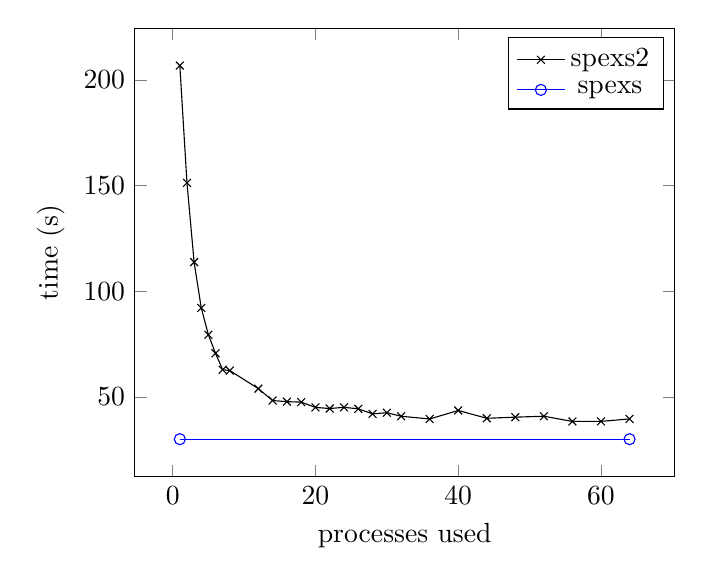
\begin{tikzpicture}
		\begin{axis}[xlabel=processes used, ylabel=time (s)]
			\addplot[color=black, mark=x] coordinates {
				(1, 206.81)
				(2, 151.30)
				(3, 113.80)
				(4, 92.16)
				(5, 79.42)
				(6, 70.66)
				(7, 62.89)
				(8, 62.49)
				(12, 53.93)
				(14, 48.30)
				(16, 47.77)
				(18, 47.56)
				(20, 45.06)
				(22, 44.53)
				(24, 45.09)
				(26, 44.39)
				(28, 41.99)
				(30, 42.55)
				(32, 40.87)
				(36, 39.58)
				(40, 43.61)
				(44, 39.91)
				(48, 40.44)
				(52, 40.89)
				(56, 38.41)
				(60, 38.45)
				(64, 39.61)
			};

			\addplot[color=blue, mark=o] coordinates {
				(1, 30.02)
				(64, 30.02)
			};

			\legend{spexs2, spexs}
		\end{axis}
	\end{tikzpicture}}
\subfloat[]{%
	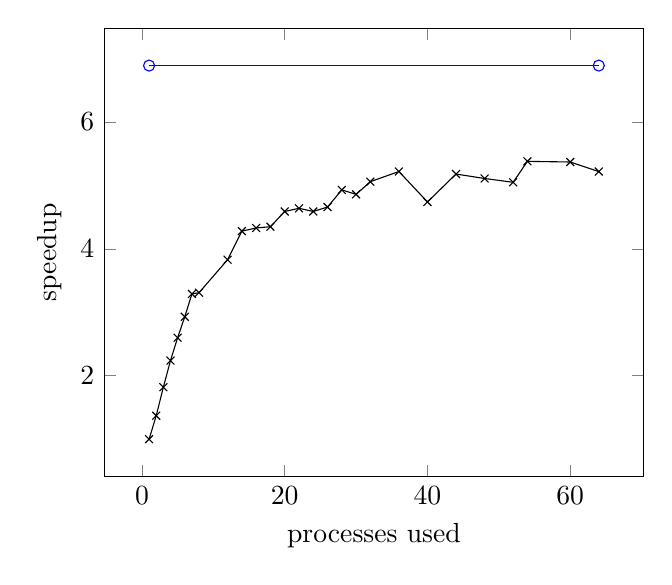
\begin{tikzpicture}
		\begin{axis}[xlabel=processes used, ylabel=speedup]
			\addplot[color=black, mark=x] coordinates {
				(1, 1.00)
				(2, 1.37)
				(3, 1.82)
				(4, 2.24)
				(5, 2.60)
				(6, 2.93)
				(7, 3.29)
				(8, 3.31)
				(12, 3.83)
				(14, 4.28)
				(16, 4.33)
				(18, 4.35)
				(20, 4.59)
				(22, 4.64)
				(24, 4.59)
				(26, 4.66)
				(28, 4.93)
				(30, 4.86)
				(32, 5.06)
				(36, 5.22)
				(40, 4.74)
				(44, 5.18)
				(48, 5.11)
				(52, 5.05)
				(54, 5.38)
				(60, 5.37)
				(64, 5.22)
			};

			\addplot[color=blue, mark=o] coordinates {
				(1, 6.89)
				(64, 6.89)
			};
		\end{axis}
	\end{tikzpicture}}
}
\end{figure}

The original \emph{spexs} works faster than \emph{spexs2} which is to be expected due to the runtime differences. At single core \emph{spexs2} performance is about 7 times slower than \emph{spexs}. We can expect 2x performance difference due to the Go runtime and compiler. The rest of the difference ~3.5x are most likely due to more general algorithm and some simplifications that were made to increase code readability.

The parallelization has significant benefit up to 20 cores. Amdahl's Law \cite{AmdahlsReval} states that the the parallel algorithms will be limited by their sequential parts; so this falloff is to be expected. The parallelization is effective, although the runtime has significant impact on the performance. \emph{spexs2} performance can be significantly improved with optimizations\footnote{The focus currently has mainly been simplicity, readability and memory usage.} that weren't implemented due to time constraints.